% Poster Coeffis 2018-2019

%--------------------------------------------------------------------
% PACKAGES AND OTHER DOCUMENT CONFIGURATIONS
%--------------------------------------------------------------------

\documentclass[a0,portrait]{a0poster} % Poster tamaño A0, orientación vertical

% Columnas
\usepackage{multicol} % Permite múltiples columnas en el documento
\columnsep=100pt % Separación entre las columnas
\columnseprule=3pt % Línea de separación entre las columnas

% Paleta de colores
%\columnseprule=3pt % Línea de separación
\usepackage[svgnames]{xcolor} % Proporciona una amplia gama de colores para utilizar en el documento. Puedes encontrar la lista completa de colores en http://www.latextemplates.com/svgnames-colors

% Fuente y lenguaje
\usepackage{times} % Usa la fuente Times
\usepackage[utf8]{inputenc} % Permite el uso de caracteres UTF-8 para acentos y otros caracteres especiales
\usepackage[spanish]{babel} % Establece el idioma del documento en español

% Texto
\usepackage[document]{ragged2e} % Proporciona una mejor justificación del texto en el documento

% Imágenes
\usepackage{graphicx,type1cm, lettrine} % Permite incluir imágenes en el documento
\usepackage[font=small,labelfont=bf]{caption} % Permite personalizar la apariencia de las leyendas de las imágenes
\usepackage{wrapfig} % Permite incluir imágenes con texto alrededor
\usepackage{subfigure} % Permite incluir varias imágenes en una misma figura
\usepackage{setspace} % Permite ajustar el espaciado entre líneas en el documento
\usepackage[left=2cm,right=2cm,top=2cm,bottom=2cm]{geometry} % Establece los márgenes del documento

% Matemáticas
\usepackage{amsfonts, amsmath, amsthm, amssymb} % Proporciona una amplia variedad de símbolos y notaciones matemáticas
\usepackage{esvect} % Permite utilizar vectores en expresiones matemáticas

% Color
\usepackage{tcolorbox} % Permite crear cajas con colores personalizados
\usepackage{xcolor} % Proporciona un conjunto de colores predefinidos
\usepackage{transparent} % Permite ajustar la opacidad de los objetos en el documento

% Crear una caja verde de resaltado
\newtcbox{\highlight}[0]{boxsep=0pt,left=0pt,top=0pt,bottom=0pt,right=0pt,boxrule=0pt,arc=0pt,auto outer arc,colback=green,width=6cm}

% Permite que las imágenes aparezcan en la posición exacta en la que se han incluido en el código
\usepackage{float}

%------------------------------------------------------------------------------------------------------------------------------------------------------------------------------%
% Fondo de pantalla configuración
%------------------------------------------------------------------------------------------------------------------------------------------------------------------------------%
\usepackage[pages=all]{background} % Permite incluir una imagen de fondo en todas las páginas del documento

% Configuración de la imagen de fondo
\backgroundsetup{
 scale=1, % Escala de la imagen. Se recomienda que sea del mismo tamaño que el documento
 color=black, % Fondo a usar para transparencia
 opacity=1, % Nivel de transparencia
 angle=0, % En caso de querer rotar la imagen de fondo
 contents={%
  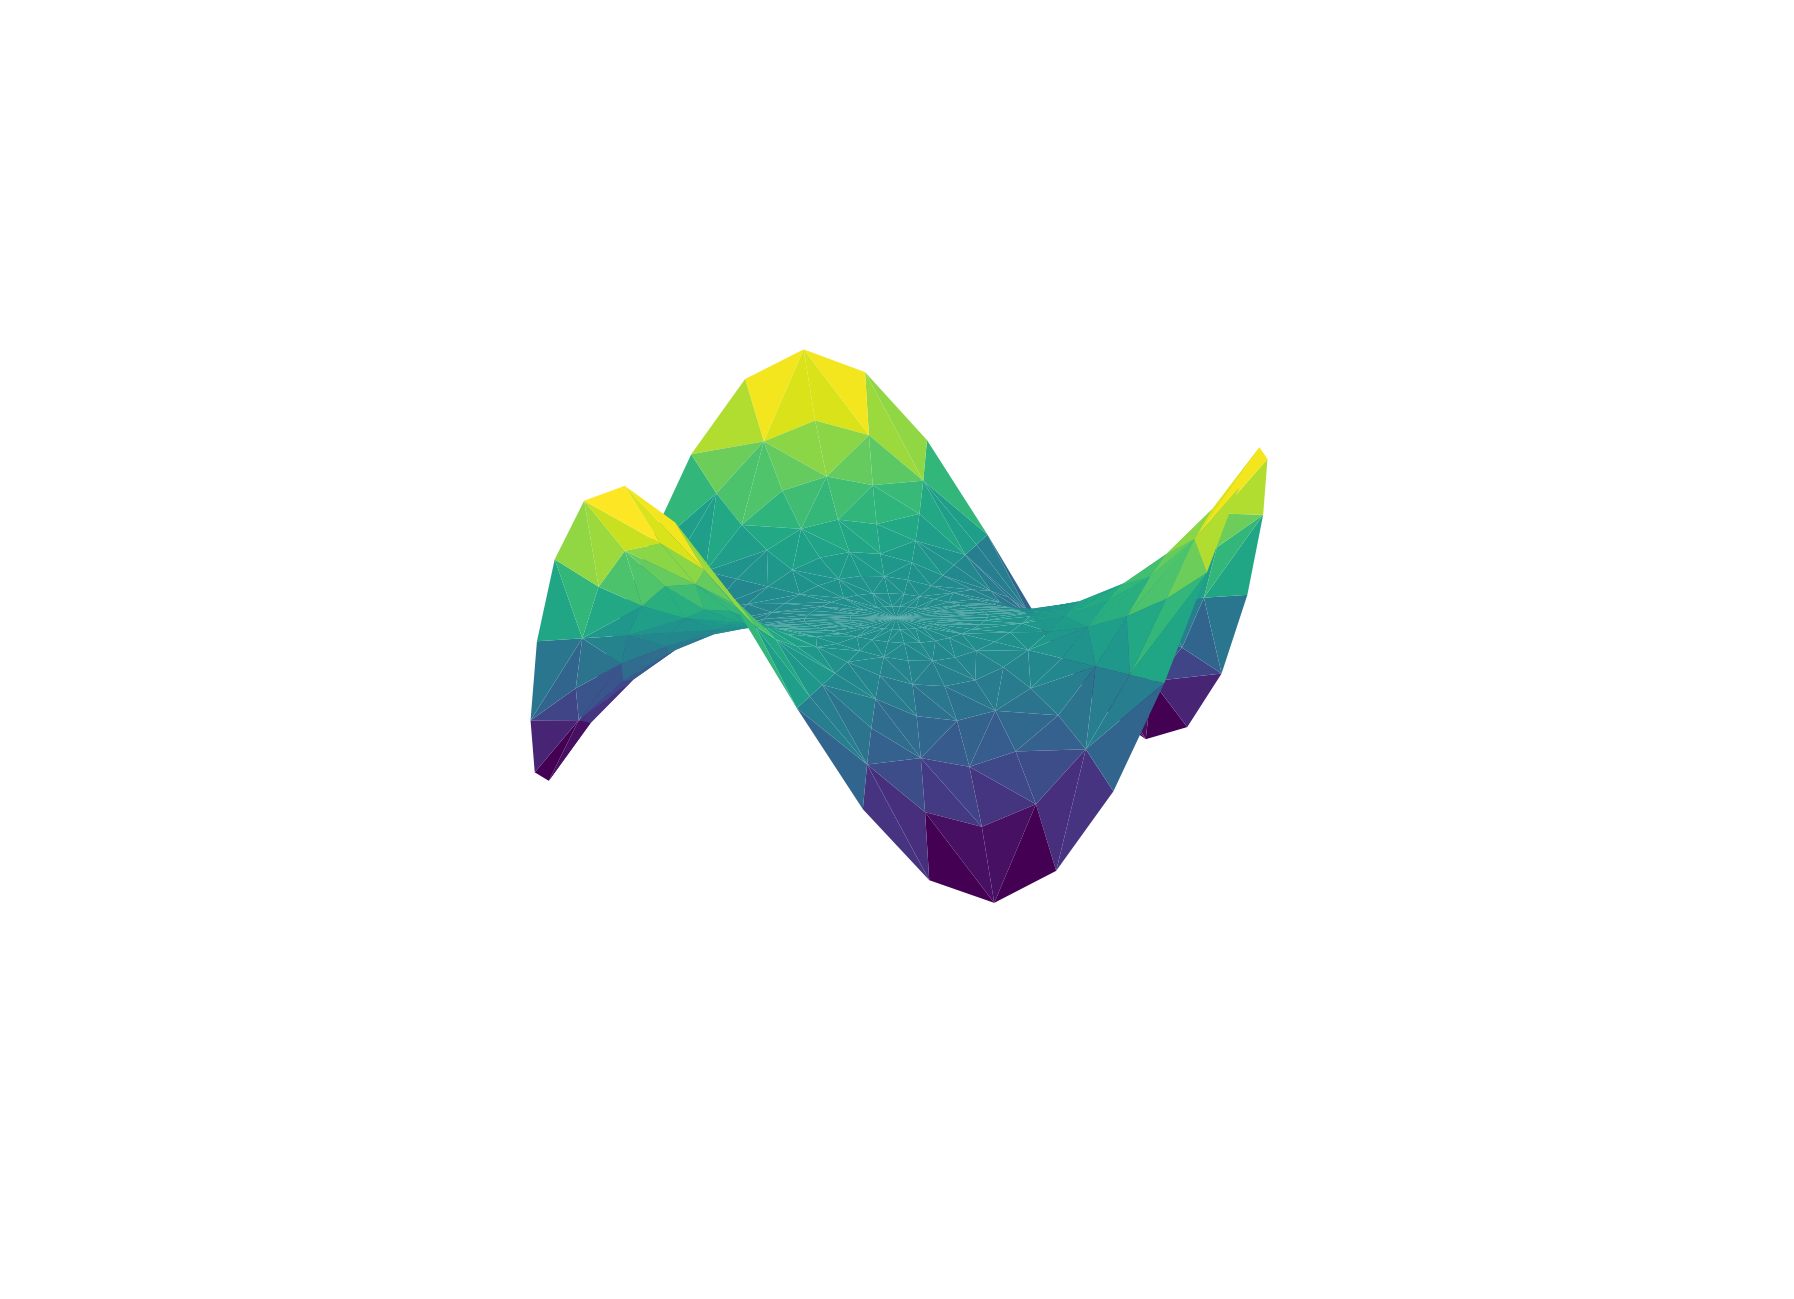
\includegraphics[width=180cm,height=140cm]{Media/Fondo_poster.png} % Nombre de la imagen a utilizar como fondo
 }%
}

\title{
\includegraphics[scale=0.5]{Media/Titulo.png}} % Título del póster
\author{\textsc{\huge Juan José Fernández Morales}} % Nombre del autor
\date{} % No se muestra la fecha

\begin{document}

\pagestyle{empty} % No se incluyen números de página en el documento
\maketitle % Crea la página de título
\thispagestyle{empty} % No se incluyen números de página en la página de título

%------------------------------------------------------------------------------------------------------------------------------------------------------------------------------%
%  Abstract del póster
%------------------------------------------------------------------------------------------------------------------------------------------------------------------------------%

\begin{center}{\fontsize{36}{40} \selectfont
    Los campos tensoriales son entidades algebraicas popularizadas por Tullio Levi-Civita con su publicación \textit{Cálculo Diferencial Absoluto} y posteriormente por Albert Einstein en su teoría de la relatividad general. El póster consta de tres partes bien diferenciadas: en la primera se definen y clasifican los tensores, en la segunda se muestran ciertas propiedades que se usan en el cálculo tensorial y finalmente se define el Tensor de Riemann-Christoffel.
    }
\end{center} 
\vspace{20pt} % Espacio entre el abstract y el resto del documento

%------------------------------------------------------------------------------------------------------------------------------------------------------------------------------%
%	Primera Parte
%------------------------------------------------------------------------------------------------------------------------------------------------------------------------------%

\begin{multicols}{2}

%------------------------------------------------------------------------------------------------------------------------------------------------------------------------------%
%	Tensor: escalar y vector
%------------------------------------------------------------------------------------------------------------------------------------------------------------------------------%
\section*{\centering Tensor: escalar y vector}

\justify{El tensor generaliza la idea de escalar o vector, independiente del sistema de coordenadas, con la capacidad de poder especificar cada una de las componentes del objeto. El tensor se puede clasificar por su orden, es decir, por el número de índices que necesita para determinar cada componente del tensor. \\[0.3cm]}

\begin{figure}[H]
    \centering
    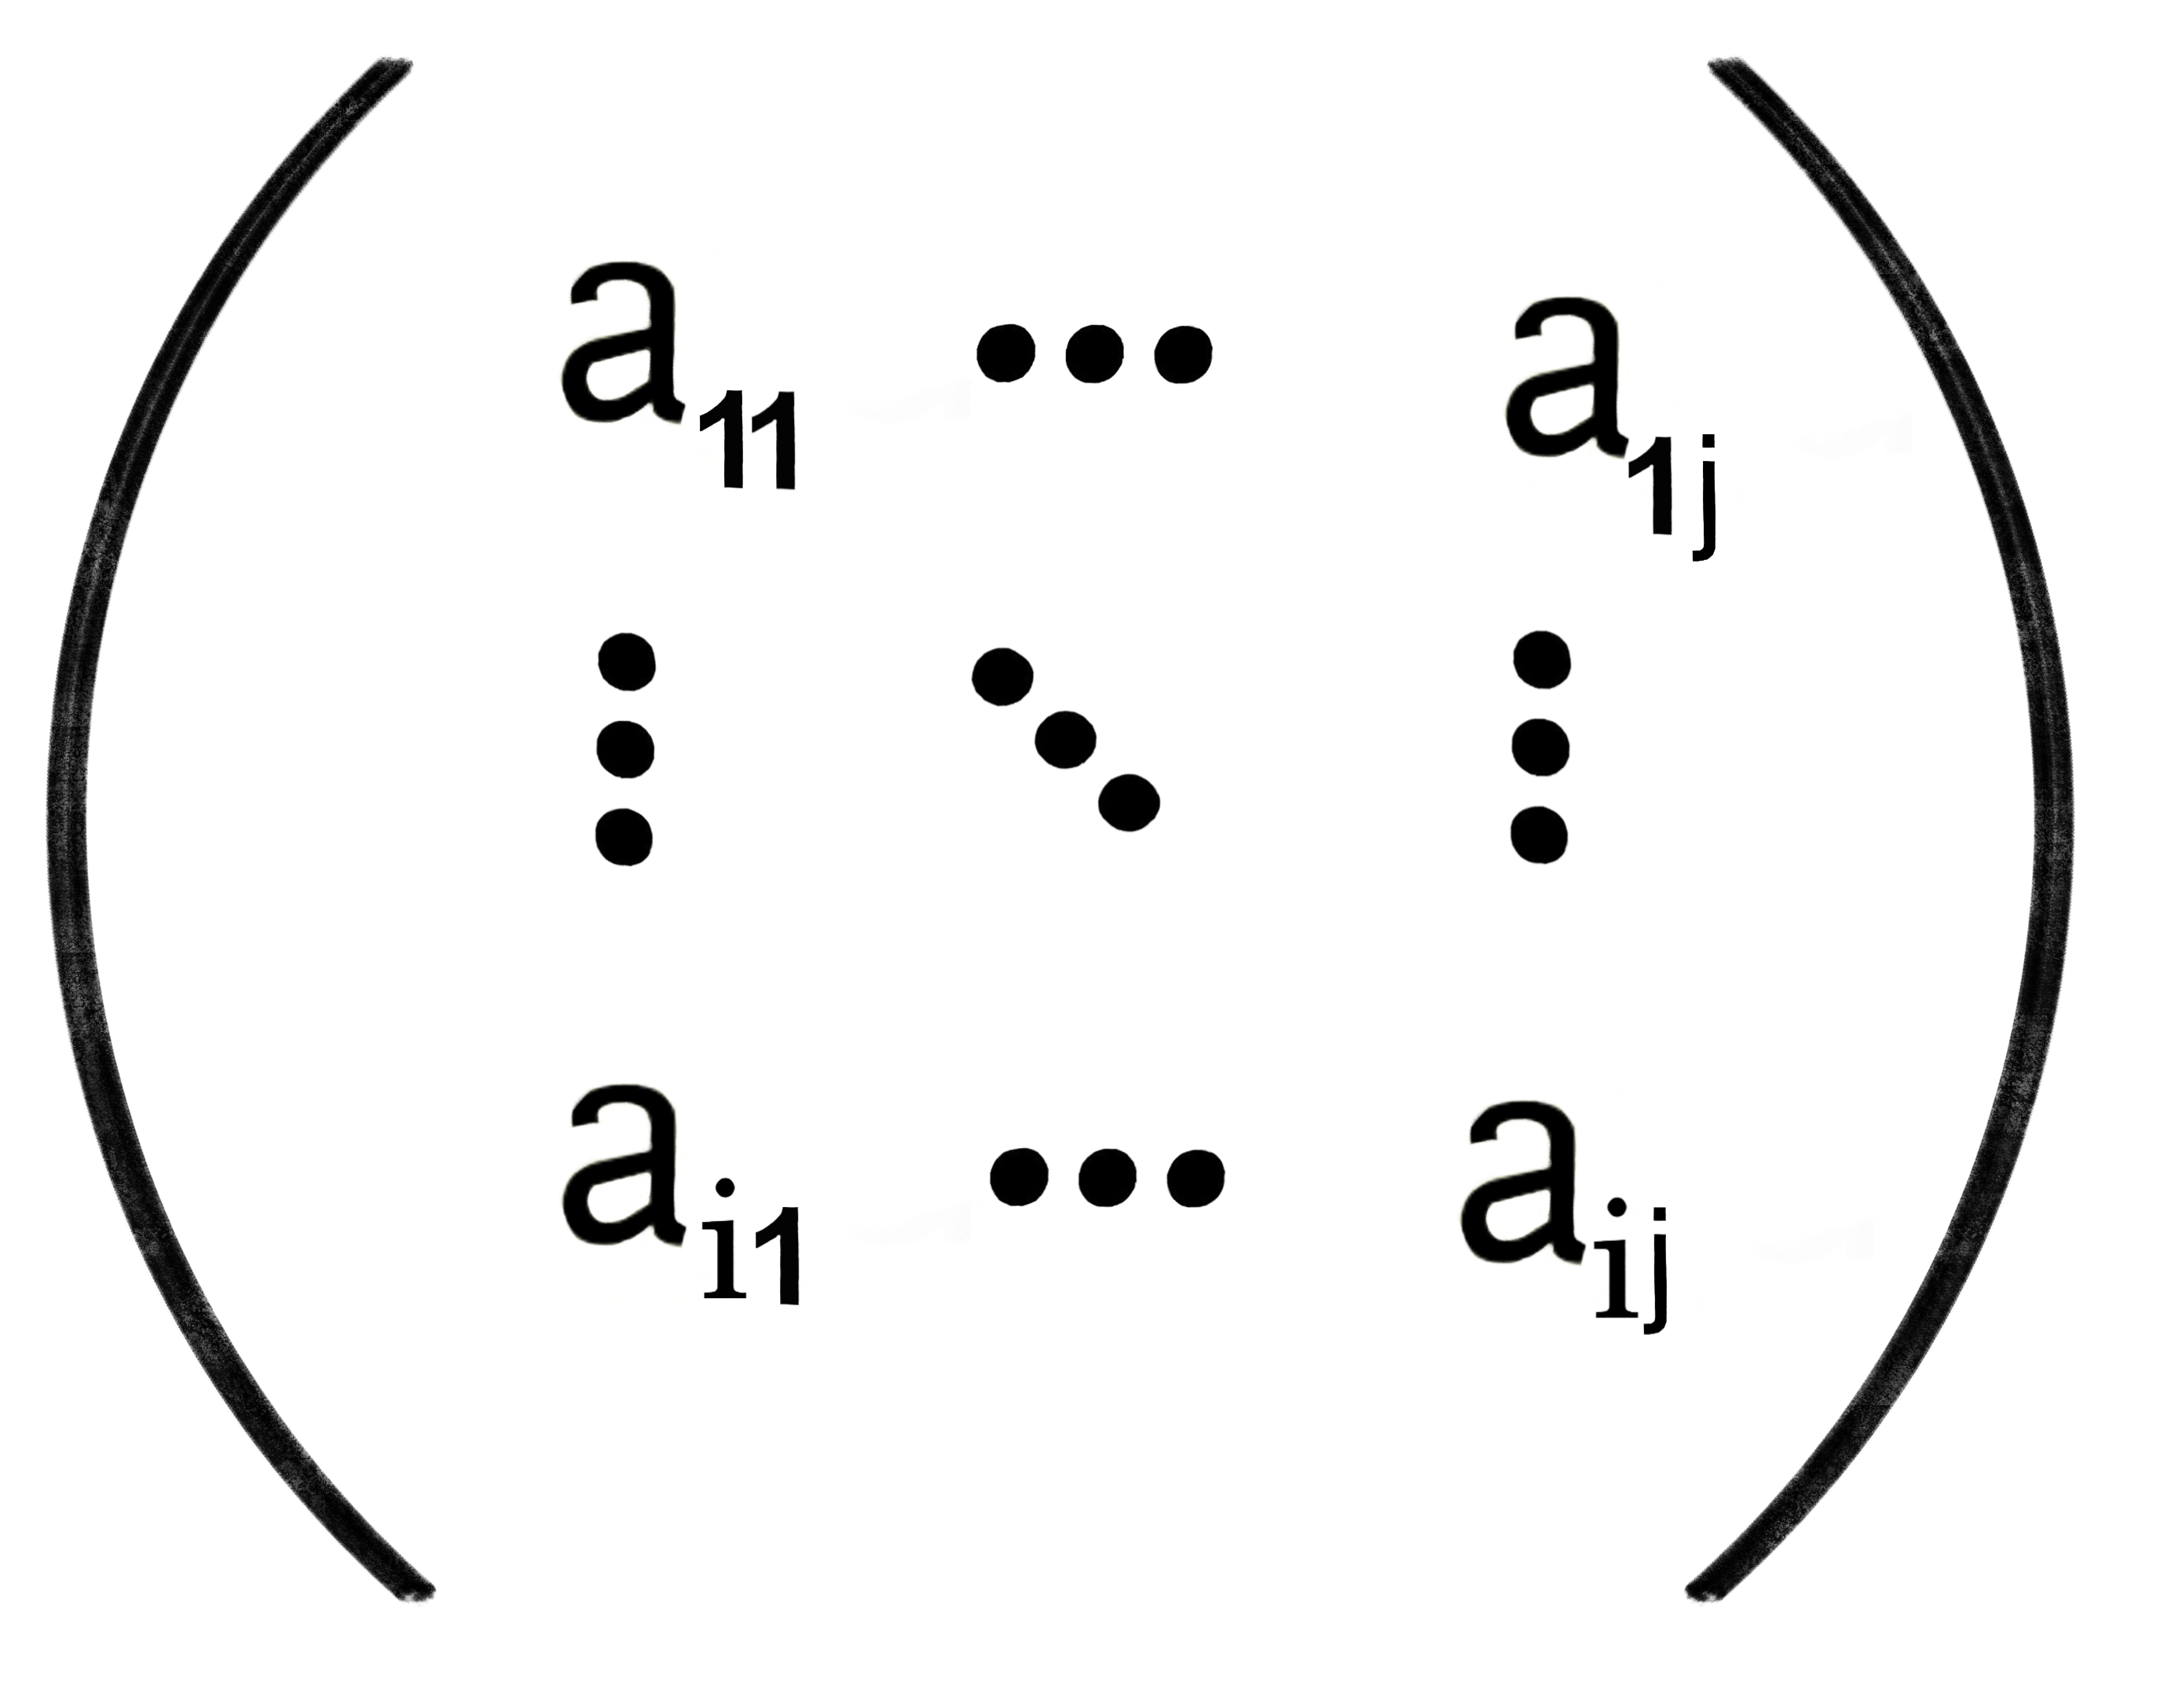
\includegraphics[scale=0.1]{Media/Matrizorden2.png}
    \caption{Forma común de expresar un tensor de orden 2 con $ij$ elementos.}
    \label{fig:MatrizOrden2}
\end{figure}

\justify{Un tensor de orden 0, comúnmente denominado escalar, no presenta ningún tipo de índice, un tensor de orden 1 se denomina vector y un tensor de orden 2 (Figura \ref{fig:MatrizOrden2}) se representa como una matriz cuadrada.\\[0.025cm]}

\textbf{\textit{Ejemplo: Los libros de una estantería podrían formar un tensor de orden 2 ($L_{ij}$), de tal forma que el segundo libro de la tercera estantería sería la componente $L_{32}$.\\[0.025cm]}}

\justify{Para el Tensor de Riemann-Christoffel, se trabajará con tensores en variedades pseudo-riemannianas. En estas variedades se puede conocer el número de elementos que presenta un tensor si se conocen las dimensiones del espacio y el orden del tensor.\\[0.25cm]}

\begin{center}
       \textit{En un espacio $\mathbb{R}^n$, un tensor de Riemann-Christoffel de orden $m$  presenta $n^m$ componentes.}
\end{center}

%------------------------------------------------------------------------------------------------------------------------------------------------------------------------------%
%	 Herramientas del cálculo tensorial}
%------------------------------------------------------------------------------------------------------------------------------------------------------------------------------%
\section*{\Centering Herramientas del cálculo tensorial}

\justify{En este apartado se explican algunas herramientas que se usan para la introducción del Tensor de Riemann-Christoffel.
En primer lugar, en el cálculo tensorial existe una  distinción del uso del subíndice ($e_j$) y el superíndice ($e^i$) (también denominados covariante y contravariante respectivamente) ya que deben cumplir la siguiente relación:}

\begin{equation}
    e_j \cdot e^i = \delta_j^i
\end{equation}

\begin{center}
    \textit{Donde} $\delta_{j}^i$  \textit{es la delta de Kronecker}\\
\end{center}

\justify{En segundo lugar, se define el tensor métrico como una función que establece la distancia entre elementos de un conjunto de vectores tangentes de una variedad diferenciable. En física se suele expresar como el cuadrado del arco entre dos elementos:}

\begin{equation}
    ds^2 = g_{ij} dx^i dx^j
\end{equation}

\textbf{\textit{Ejemplo: de un elemento de arco \textbf{en esféricas} se puede obtener su tensor métrico:}

\begin{equation*}
    ds^2 = dr^2 + r^2d\theta^2 + r^2\sin{\theta}^2d\phi^2 \rightarrow g = 
    \begin{vmatrix}
        1&0&0\\
        0&r^2&0\\
        0&0&r^2\sin{\theta}^2
        \\
    \end{vmatrix}
\end{equation*}}

%Imagen de una gráfica en esféricas

\justify{Por último, la derivada covariante generaliza la derivada parcial. Se trata de una herramienta fundamental para el cálculo diferencial en variedades diferenciables. Se representa como $\nabla_i$ y se define como:}

\begin{equation}
    \nabla_i\vec{A} = \frac{\partial(A^je_j)}{\partial x^i} = \frac{\partial A^j}{\partial x^i}e_j+A^j\frac{\partial e_j}{\partial x^i} = (\partial_i A^j)e_j + A^j(\partial_i e_j)
\end{equation}

\justify{La variación de un elemento de la base se define con los símbolos de Christoffel ($\Gamma^k_{i j}$), aunque estos símbolos también se pueden definir mediante la métrica:}

\begin{gather}
    \Gamma^k_{i j} = (\partial_i e_j)e^k; k = 1, \cdots, n\\
    \Gamma^k_{i j} = \frac{1}{2}g^{km}(\partial_j g_{mi}+\partial_i g_{m j}-\partial_m g_{ji})
\end{gather}

Por lo que la derivada covariante también se puede expresar como:

\begin{equation}
    \nabla_i \vec{A} = (\partial_i A^k+\Gamma^k_{i j}A^j)e_k
\end{equation}

% Observasión
\textbf{\justify{\textit{Observación}: Si la base no varia con respecto a la coordenada i-ésima ($\Gamma^k_{i j} = 0$), entonces la derivada covariante se comporta igual que la derivada parcial convencional:}}

\begin{equation*}
    \nabla_i\vec{A} = \frac{\partial A^j}{\partial x^i}e_j
\end{equation*}

%------------------------------------------------------------------------------------------------------------------------------------------------------------------------------%
%	Segunda Parte
%------------------------------------------------------------------------------------------------------------------------------------------------------------------------------%

\end{multicols}
\vspace{1cm}
\section*{\Centering Tensor de Riemann-Christoffel}

\columnseprule=3pt
\begin{multicols}{3}

\justify{El Tensor de Riemann-Christoffel ($R^i_{jkl}$) es un tensor de orden 4, con 1 índice contravariante y 3 índices covariantes (de tipo $(1, 3)$). Este objeto se emplea para obtener información de la curvatura de cualquier variedad riemanniana (o pseudoriemanniana) de un espacio n dimensional.\\}

\begin{figure}[H]
    \centering
    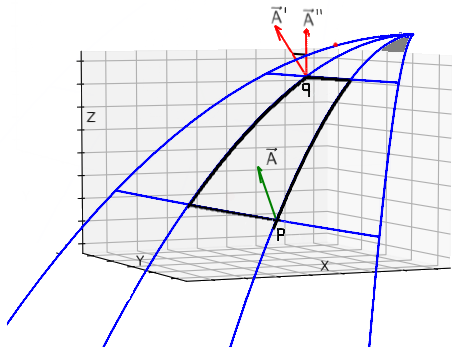
\includegraphics[scale=1.3]{Media/Transporte_paralelo.png}
    
    \caption{\centering Transporte paralelo del vector $\vec{A}$ desde el punto $p$ en una variedad (azul) a través de un trayectoria (negra)}
    \label{fig:transporte_paralelo}
\end{figure}

\justify{Para mostrar como se comporta, que información da y como se obtiene se precede a realizar una pequeña demostración:}

\justify{En una variedad diferenciable sin torsión de un espacio pseudoriemanniano $n$ dimensional, se obtiene el tensor de Riemann-Christoffel como la diferencia de dos resultantes del transporte paralelo de un punto $p$ a un punto $q$ de un vector $\vec{A}$, por dos caminos distintos de una trayectoria cerrada que varía de forma bien definida por cada componente de la base de la variedad (Figura \ref{fig:transporte_paralelo}).}

\justify{Si se expresa de forma matemática, en base a la notación de Einstein para la suma, se tendría que:}

\begin{equation}
    R^i_{jkl}A^j = \nabla_k\nabla_l A^i - \nabla_l \nabla_k A^i \\
\end{equation}

\justify{Se estudia uno de los términos de la diferencia, ya que se trata de las mismas expresiones pero con las variables cambiadas. Si se usa la expresión obtenida en el apartado anterior, se tiene que:}

\begin{multline}
    \nabla_k\nabla_lA^i= \partial^2_{kl}A^i+(\partial_k\Gamma^i_{lj})A^j+\Gamma^i_{lj}\partial_kA^j+ \\ +\Gamma^i_{kj}\partial_lA^j+\Gamma^i_{kj}\Gamma^j_{ln}A^n-\Gamma^j_{kl}\partial_jA^i-\Gamma^j_{kl}\Gamma^i_{jm}A^m
\end{multline}

\justify{Al sustituir en la diferencia, aplicar el Teorema de Schwarz ($\partial_i\partial_jA = \partial_j\partial_iA$) y suponer que los símbolos de Christoffel son simétricos ($\Gamma^i_{kj} = \Gamma^i_{jk}$) queda la siguiente expresión:}

\begin{equation}
        R^i_{jkl}A^j = (\partial_k\Gamma^i_{lj}-\partial_l\Gamma^i_{kj}+\Gamma^i_{kn}\Gamma^n_{lj}-\Gamma^i_{ln}\Gamma^n_{kj})A^j
\end{equation}

\subsection* {Tensor de Ricci y curvatura escalar de Ricci}

\justify{Como corolario se pueden obtener el Tensor de Ricci y la curvatura escalar de Ricci:\\}

\justify{El tensor de Riemann-Christoffe se puede particularizar para variedades que se encuentren en un espacio de dimensión $n \leq 4$, al contraer un índice covariante y otro contravariante, en este caso al igualar el superíndice $i$ con el subíndice $k$ (con la suma que implica sobre el índice repetido). Esta particularización se denomina Tensor de Ricci.}

\begin{equation}
    R^k_{jkl} := R_{jl}
\end{equation}

\begin{center}
    \textit{
            El Tensor de Ricci es un tensor de orden 2, tipo (0,2).
            }
\end{center}

Como ejemplo, si se toma la expresión (9):

\begin{equation}
    R^k_{jkl} = \partial_k\Gamma^k_{lj}-\partial_l\Gamma^k_{kj}+\Gamma^k_{kn}\Gamma^n_{lj}-\Gamma^{k}_{ln}\Gamma^n_{kj}
\end{equation}

\justify{A su vez, en el Tensor de Ricci se pueden contraer los dos subíndices restantes. El parámetro que se obtiene permite definir la curvatura de una variedad de un espacio de dimensión $n \leq 2$. A este objeto se le denomina Escalar de Ricci.}

\begin{equation}
    R := g^{ij}R_{ij}
\end{equation}
\begin{center}
    \textit{
            La curvatura escalar de Ricci es un tensor de orden 0, un escalar.
            }
\end{center}

\end{multicols}
\vspace{1cm}



\columnseprule=0pt
\begin{multicols}{2}

\textbf{\large{\justify{Una de las aplicaciones más populares de estos objetos es en la teoría de la Relatividad General de Einstein, por ejemplo, la ecuación del campo de Einstein se describe de la siguiente forma:}}}

\large{
\begin{equation*}
    R_{\mu \nu} - \frac{1}{2}Rg_{\mu \nu} + \lambda g_{\mu \nu} = \frac{8\pi G}{c^4}T_{\mu \nu}
\end{equation*}}

\textbf{
\large{
\justify{
Donde $R_{\mu \nu}$ el tensor de Ricci, $R$ la curvatura escalar de Ricci, $g_{\mu \nu}$ la métrica, $\lambda$ la constante cosmológica, $T_{\mu \nu}$ es el tensor de energía-momento, c la constante de la velocidad de la luz y G la constante gravitacional.}}}


\begin{figure}[H]
    \centering
    
\includegraphics{Media/logo_coefis_negro.png}
\end{figure}
\end{multicols}

\vspace{2cm} 
\columnsep=300px
\begin{multicols}{2}
\small{
\begin{thebibliography}{6}
\bibitem{Relatividad1}
Bernan F. Schutz.
\textit{A First Course in General Relativity}.
(CAMBRIDGE UNIVERSITY PRESS), 2015.

\bibitem{Relatividad2}
J. Lelong-Ferrand.
\textit{Géométrie Différentielle}.
MASSON et Cie, 1963.

\bibitem{Tensor1}
David Lovelock and Hanno Rund.
\textit{Tensors, Differential Forms and Variational Principles}
Dover, 1975.

\bibitem{Tensor2}
Javier Garcia (Canal de Youtube)
\text{16 - Curso de Relatividad General [Tensor de Riemann]}, 2018.

\bibitem{Tensor3}
Dan Fleisch (Canal de Youtube).
\textit{What's a tensor?}, 2011.

\bibitem{Tensor4}
Ingeniero Electrónico (Canal de Youtube)
\text{54 Cálculo Tensorial XIV. Tensor de Riemann}, 2015.
\end{thebibliography}}
\end{multicols}

\end{document}